\section[Lezione 22 - Fattorizzazione LU]{Lezione 22 - MEG come prodotto per matrici elementari di trasformazione, fattorizzazione LU di una matrice non singolare}
Nella scorsa lezione abbiamo discusso del metodo di eliminazione gaussiana come metodo di riduzione di una matrice quadrata non singolare a forma \uline{triangolare}, che permette di usarlo per calcolare il determinante (nel caso singolare ci si accorge durante l'esecuzione che il determinante è nullo).\\In particolare abbiamo studiato l'implementazione in aritmetica floating-point con la tecnica del \uline{pivoting}, che permette di superare il problema della comparsa di un elemento nullo sulla diagonale e dal punto di vista numerico ha un effetto \uline{stabilizzante} sull'algoritmo (evitando la generazione di numeri arrotondati troppo grandi e quindi limitando la perdita di precisione nelle sottrazioni).\\
Sia l'operazione fondamentale di \uline{annullamento} che l'operazione di \uline{scambio} legata al pivoting si possono in realtà scrivere in \uline{forma matriciale}, come prodotto a sinistra per opportune \uline{matrici elementari} di trasformazione.

\subsection{Scambio di due righe}
Cominciamo con lo scambio di 2 righe: lo scambio della riga $k$ con la riga $i$ di una generica matrice $B\in\mathbb{R}^{n\times n}$ si ottiene moltiplicando a sinistra $B$ per la matrice identità in cui sono state scambiate le righe $k$ e $i$ (chiameremo $S_{k,i}$ tale matrice).\\Facciamo un esempio $3\times 3$
\begin{equation*}
    S_{2,1}B=
    \begin{pmatrix}
        0 & 1 & 0 \\
        1 & 0 & 0 \\
        0 & 0 & 1
    \end{pmatrix} \cdot \begin{pmatrix}
        b_{11} & b_{12} & b_{13} \\
        b_{21} & b_{22} & b_{23} \\
        b_{31} & b_{32} & b_{33}
    \end{pmatrix}=\begin{pmatrix}
        b_{21} & b_{22} & b_{23} \\
        b_{11} & b_{12} & b_{13} \\
        b_{31} & b_{32} & b_{33}
    \end{pmatrix}
\end{equation*}
ha esattamente l'effetto di scambiare la riga 2 con la riga 1 di $B$.\\Si osservi che $det(S_{2,1})=-1$ e che $S_{2,1}\cdot S_{2,1}= I$ cioè $S_{2,1}^{-1}=S_{2,1}$.\\
In generale
\[
    S_{k,i}=\begin{blockarray}{ccccccccc}
        & & & \matindex{i} & &  \matindex{k} & & \\
        \begin{block}{(cccccccc)c}
        1 & 0 & \dots & 0 & \dots & 0 & \dots & 0 \\
        0 & 1 & \dots & 0 & \dots & 0 & \dots & 0 \\
        \vdots & \vdots &  & \vdots &  & \vdots &  & \vdots \\
        0 & 0 & \dots & 0 & \dots & 1 & \dots & 0 & \matindex{i} \\
        \vdots & \vdots &  & \vdots &  & \vdots &  & \vdots \\
        0 & 0 & \dots & 1 & \dots & 0 & \dots & 0 & \matindex{k} \\
        \vdots & \vdots &  & \vdots &  & \vdots &  & \vdots \\
        0 & 0 & \dots & 0 & \dots & 0 & \dots & 1 \\
        \end{block}
    \end{blockarray}
\]
e \quad $S^{-1}_{k,i}=S_{k,i}$, \quad   $det(S_{k,i})=-1$.\\Quest'ultima uguaglianza spiega in forma matriciale perchè scambiare 2 righe cambia segno al determinante, ricordando che il determinante del prodotto di due matrici è il prodotto dei determinanti 
\begin{equation*}
    det(S_{k,i}B)=det(S_{k,i})det(B)=-det(B)
\end{equation*}

\subsection{Moltiplicazione tra due righe}
L'altra operazione vettoriale chiave del $meg$ al passo i-esimo è
\begin{equation*}
    \mathcal{R}^{(i+1)}_k:=\mathcal{R}^{(i)}_k+(\overbrace{-m_{ki}}^{moltiplicatore})\mathcal{R}^{(i)}_i
\end{equation*}
dove $m_{ki}=\frac{a_{ki}^{(i)}}{a_{ii}^{(i)}}$, $i+1\leq k\leq n$, detto ``\uline{moltiplicatore}" ha lo scopo di propagare la struttura di zeri
\begin{center}
    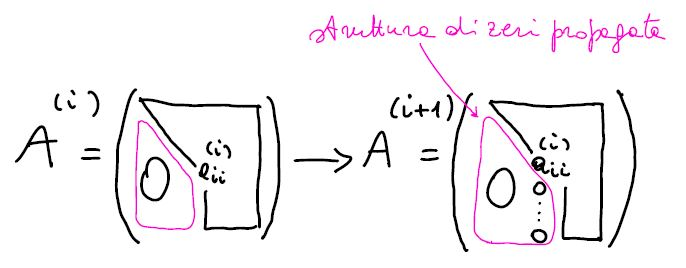
\includegraphics[scale=0.5]{foto/calcolo_2.JPG}    
\end{center}
In generale l'operazione tra righe
\begin{equation*}
    \mathcal{R}_k:=\mathcal{R}_k+\alpha\mathcal{R}_i
\end{equation*}
di una matrice $B\in\mathbb{R}^{n\times n}$ corrisponde a moltiplicare a sinistra per la matrice elementare
\[
    T_{k,i}=\begin{blockarray}{ccccccccc}
    & & & \matindex{i} & &  \matindex{k} & & \\
        \begin{block}{(cccccccc)c}
        1 & 0 & \dots & 0 & \dots & 0 & \dots & 0 \\
        0 & 1 & \dots & 0 & \dots & 0 & \dots & 0 \\
        \vdots & \vdots &  & \vdots &  & \vdots &  & \vdots \\
        0 & 0 & \dots & 1 & \dots & 0 & \dots & 0 & \matindex{i} \\
        \vdots & \vdots &  & \vdots &  & \vdots &  & \vdots \\
        0 & 0 & \dots & \alpha & \dots & 1 & \dots & 0 & \matindex{k} \\
        \vdots & \vdots &  & \vdots &  & \vdots &  & \vdots \\
        0 & 0 & \dots & 0 & \dots & 0 & \dots & 1 \\
        \end{block}
    \end{blockarray}
\]
che si ottiene dalla matrice identità mettendo $\alpha$ al punto di 0 come elemento $k,i$.\\Facciamo un esempio $3\times 3$
\begin{equation*}
    T_{3,1}(\alpha)B=
    \begin{pmatrix}
        1 & 0 & 0 \\
        0 & 1 & 0 \\
        \alpha & 0 & 1
    \end{pmatrix} \cdot \begin{pmatrix}
        b_{11} & b_{12} & b_{13} \\
        b_{21} & b_{22} & b_{23} \\
        b_{31} & b_{32} & b_{33}
    \end{pmatrix}=\begin{pmatrix}
        b_{11} & b_{22} & b_{33} \\
        b_{21} & b_{22} & b_{23} \\
        \alpha b_{11}+b_{31} & \alpha b_{12}+b_{32} & \alpha b_{13}+b_{33}
    \end{pmatrix}
\end{equation*}
Si osservi che si tratta di una matrice triangolare inferiore con 1 sulla diagonale principale e quindi $det(T_{k,i}(\alpha))=1$ e che $T_{k,i}(-\alpha)T_{k,i}(\alpha)= I$ cioè $(T_{k,i}(\alpha))^{-1}=T_{k,i}(-\alpha)$.\\Infatti, tornando per fissare le idee all'esempio $3\times 3$
\begin{equation*}
    T_{3,1}(-\alpha)T_{3,1}(\alpha)=
    \begin{pmatrix}
        1 & 0 & 0 \\
        0 & 1 & 0 \\
        -\alpha & 0 & 1
    \end{pmatrix} \cdot \begin{pmatrix}
        1 & 0 & 0 \\
        0 & 1 & 0 \\
        \alpha & 0 & 1
    \end{pmatrix}=\begin{pmatrix}
        1 & 0 & 0 \\
        0 & 1 & 0 \\
        \alpha(-\alpha) & 0 & 1
    \end{pmatrix}=\begin{pmatrix}
        1 & 0 & 0 \\
        0 & 1 & 0 \\
        0 & 0 & 1
    \end{pmatrix}
\end{equation*}
Diventa chiaro che il passo i-esimo del $meg$ si può scrivere come composizione di trasposizioni elementari tramite il prodotto a sinistra per la sequenza di matrici elementari che realizzano l'eventuale scambio del pivoting e gli annullamenti successivi in colonna $i$ sotto la diagonale.\\Prendendo l'esempio $3\times 3$ della scorsa lezione
\begin{equation*}
    A^{(1)}=A=\begin{pmatrix}
        1 & 2 & 1 \\
        \overbrace{2}^{pivot} & 2 & 3 \\
        -1 & -3 & 0
        \end{pmatrix}
\end{equation*}
abbiamo (stavolta applichiamo il pivoting per coerenza con l'implementazione anche se operiamo con frazioni)
\begin{center}
    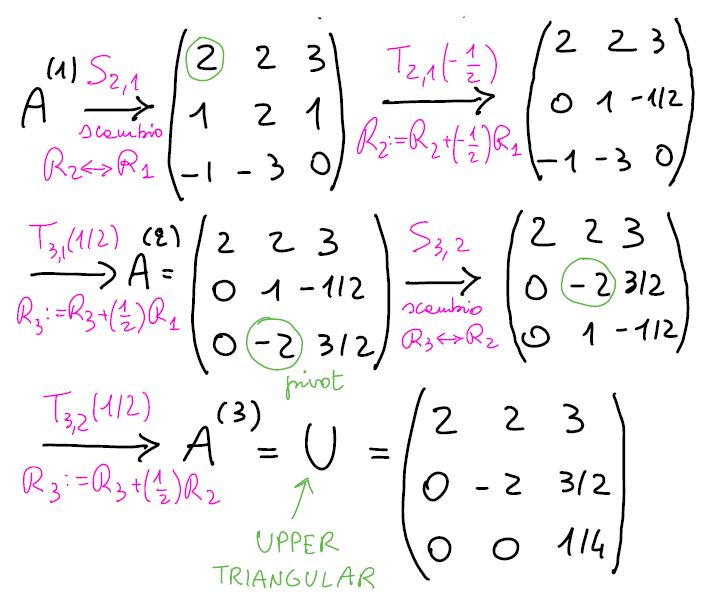
\includegraphics[scale=0.5]{foto/calcolo1_2.JPG}    
\end{center}
cioè
\[
U = A^{(3)} = T_{3,2} (\frac{1}{2}) \ S_{3,2} \underbrace{\ T_{3,1} (\frac{1}{2}) \ T_{2,1} (-\frac{1}{2}) \ S_{2,1} A}_{A^{(2)}}
\]
dove $-m_{3,2} = -m_{3,1} = \frac{1}{2}, \ -m_{2,1} = -\frac{1}{2}$ e $det(U) = 2(-2)\frac{1}{4} = -1 = det(A)$ essendoci stato un numero pari di scambi.\\
In generale si avrà che il passo i-esimo del meg in forma matriciale diventa
\[
    A^{(i+1)} = T_{n,i} (-m_{n, i}) \ T_{n-1, i} (-m_{n-1, i}) \dotso T_{i+2, i} (-m_{i+2, i})\ T_{i+1, i} (-m_{i+1, i}) \ S_{p_i, i} \ A^{(i)}
\]
con $p_i$ l'indice del pivot sottodiagonale in colonna $i$, mentre la sequenza completa di trasformazioni (A non singolare) è
\[
\begin{split}
    & U = A^{(n)} = T_{n, n-1} (-m_{n, n-1}) \ S_{p_{n-1}, n-1} \\
    & T_{n, n-2} (-m_{n, n-2}) \ T_{n-1, n-2} (-m_{n-1, n-2}) \ S_{p_{n-2}, n-2} \\
    & \dotso \ S_{p_2, 2} \ T_{n,1} (-m_{n,1}) \ \dotso \ T_{2,1} (-m_{2,1}) \ S_{p_1, 1} \ A
\end{split}
\]

\subsection{MEG come fattorizzazione $PA=LU$}
A questo punto possiamo far vedere che il meg permette di ottenere una fattorizzazione della matrice di partenza (a meno di una permutazione delle righe) nel prodotto di due matrici triangolari, una triangolare inferiore per una triangolare superiore.\\
Per semplicità ci limitiamo al caso ``senza scambi", cioè in cui il pivoting trova l'elemento di max modulo già sulla diagonale.\\
Ci sono classi di matrici per cui si può dimostrare che questo vale (lo accettiamo), ad esempio:
\begin{itemize}
    \item matrici a \uline{diagonale strettamente dominante}
    \[
        \abs{a_{ii}} > \sum_{j \neq i} \abs{a_{ij}} \  \  \  \ \forall i
    \]
    
    \item matrici \uline{simmetriche definite positive}. \end{itemize} Limitiamoci per capire meglio a matrici $3 \times 3$ con
    \[
    U = A^{(3)} = T_{3,2} (-m_{3,2}) \ T_{3,1} (-m_{3,1}) \ T_{2,1} (-m_{2,1}) \ A
    \]
    Posto $\mathcal{L} = T_{3,2} (-m_{3,2}) \ T_{3,1} (-m_{3,1}) \ T_{2,1} (-m_{2,1})$ abbiamo
    \[
    U = \mathcal{L}A \Rightarrow A = LU \ \text{con} \ L = \mathcal{L}^{-1}
    \]
    Ma come è fatta $L$?
    \[
    \begin{split}
        L = \mathcal{L}^{-1} & = \overbrace{(T_{2,1} (-m_{2,1}))^{-1} \ (T_{3,1} (-m_{3,1}))^{-1} \ (T_{3,2} (-m_{3,2}))^{-1}}^{\text{ordine invertito}} \\
        & = T_{2,1} (m_{2,1}) \ T_{3,1} (m_{3,1}) \ T_{3,2} (m_{3,2})
    \end{split}
    \]
    ricordando che $(T_{k,i} (\alpha))^{-1} = T_{k, i} (-\alpha)$ cioè
    \[
    \begin{split}
        L &=
        \begin{pmatrix}
        1 & 0 & 0 \\
        m_{2,1} & 1 & 0 \\
        0 & 0 & 1
        \end{pmatrix}
        \begin{pmatrix}
        1 & 0 & 0 \\
        0 & 1 & 0 \\
        m_{3,1} & 0 & 1
        \end{pmatrix}
        \begin{pmatrix}
        1 & 0 & 0 \\
        0 & 1 & 0 \\
        0 & m_{3,2} & 0
        \end{pmatrix} \\
        &=
        \begin{pmatrix}
        1 & 0 & 0 \\
        m_{2,1} & 1 & 0 \\
        m_{3,1} & 0 & 1
        \end{pmatrix}
        \begin{pmatrix}
        1 & 0 & 0 \\
        0 & 1 & 0 \\
        0 & m_{3,2} & 1
        \end{pmatrix}
        =
        \begin{pmatrix}
        1 & 0 & 0 \\
        m_{2,1} & 1 & 0 \\
        m_{3,1} & m_{3,2} & 1
        \end{pmatrix}
    \end{split}
    \]
    ovvero $L$ è una matrice triangolare inferiore (Lower Triangular in inglese)
    \[
    L =
    \begin{pmatrix}
    l_{11} & 0 & 0 \\
    l_{21} & l_{22} & 0 \\
    l_{31} & l_{32} & l_{33}
    \end{pmatrix}
    \]
    che ha $l_{ii} = 1, \ l_{ki} = m_{k,i}$ per $i+1 \le k \le n$ e $l_{ki} = 0$ per $k<i$
Questo è vero anche in generale
\[
L=
\begin{pmatrix}
1 & 0 & 0 & \cdots & 0 \\
m_{2,1} & 1 & 0 & \cdots & 0 \\
m_{3,1} & m_{3,2} & 1 & \cdots & 0 \\
\vdots & \vdots & \vdots & \ddots & \vdots \\
m_{n,1} & m_{n,2} & m_{n,3} & \cdots & 1
\end{pmatrix}
\]
in cui il triangolo sotto la diagonale principale contiene i moltiplicatori del meg.\\
In presenza di scambi imposti dal pivoting, si può dimostrare (non richiesto) che il meg produce comunque una fattorizzazione del tipo
\begin{center}
    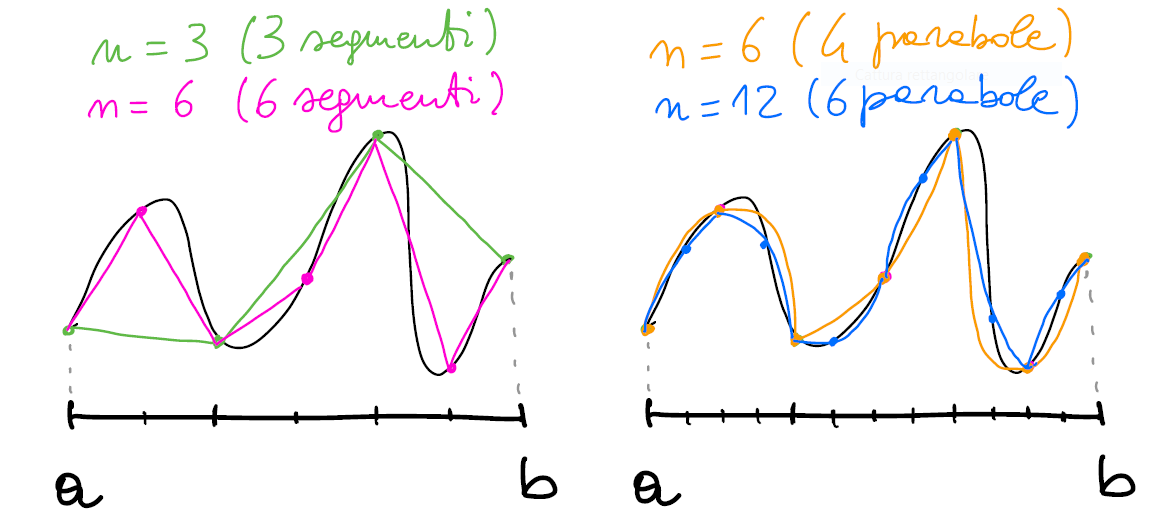
\includegraphics[width = 0.5\textwidth]{foto/pag17}
\end{center}
dove
\begin{itemize}
    \item $U$ è la matrice \uline{triangolare superiore} ottenuta alla fine del meg
    
    \item $P$ è una \uline{matrice di permutazione}
cioè una matrice invertibile che contiene solo 0 o 1 ed è ottenuta come \uline{prodotto} di matrici di \uline{scambio}.
\[ \begin{split}
	P=S_{p_{n-1},n-1} \cdot S_{p_{n-2},n-2} \cdot ... \cdot S_{p_{2},2} \cdot S_{p_{1},1}
\end{split} \]
Ad esempio nel caso $3 \times 3$, $P$ può essere:
\[ \begin{split}
	& P=I, \quad P=S_{2,1}=
		\begin{pmatrix}
		0 & 1 & 0 \\
		1 & 0 & 0 \\
		0 & 1 & 0 \\
		\end{pmatrix}
	, \quad P=S_{3,1}=
		\begin{pmatrix}
		0 & 0 & 1 \\
		0 & 1 & 0 \\
		1 & 0 & 0 \\
		\end{pmatrix}
	\\
	& P=S_{2,1}S_{3,2}=
		\begin{pmatrix}
		0 & 1 & 0 \\
		0 & 0 & 1 \\
		1 & 0 & 0 \\
		\end{pmatrix}
	, \quad P=S_{3,1}S_{3,2}=
		\begin{pmatrix}
		0 & 0 & 1 \\
		1 & 0 & 0 \\
		0 & 1 & 0 \\
		\end{pmatrix}
	\\
	& P=S_{3,2}=
		\begin{pmatrix}
		1 & 0 & 0 \\
		0 & 0 & 1 \\
		0 & 1 & 0 \\
		\end{pmatrix}
\end{split} \]
\item L è una matrice \uline{triangolare inferiore} con $l_{i\,i}=1$ $\forall i$ e con $i$ moltiplicatori opportunamente rimescolati nel triangolo inferiore sotto la diagonale (accettiamo questo fatto senza dimostrarlo per semplicità).
\end{itemize}
Quindi l'aspetto è:
\[ \begin{split}
	U=
		\begin{pmatrix}
		u_{1\,1} & .. & .. & u_{1\,n} \\
		0 & u_{2\,2} & .. & u_{2\,n} \\
		.. & .. & .. & .. \\
		0 & 0 & 0 & u_{n\,n}
		\end{pmatrix}
	, \quad L=
		\begin{pmatrix}
		1 & 0 & .. & 0 & 0 \\
		l_{2\,1} & 1 & .. & 0 & 0 \\
		.. & .. & .. & .. & .. \\
		l_{n\,1} & l_{n\,2} & .. & l_{n\,n-1} & 1 
		\end{pmatrix}
	\quad u_{i\,i} \neq 0 \; \forall i
\end{split} \]
\begin{center}
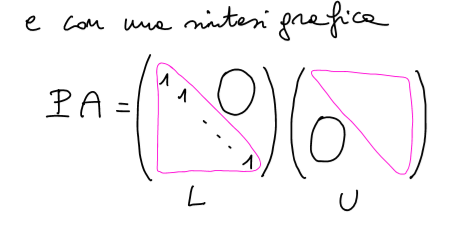
\includegraphics[width = 0.5\textwidth]{foto/pag_19}
\end{center}
Perchè le fattorizzazioni sono importanti? Perchè permettono di decomporre una matrice senza struttura nel prodotto di matrici strutturate. Nella prossima lezione vedremo infatti come risolvere sistemi lineari tramite la fattorizzazione $LU$ generata dal meg.\\\\
Concludiamo la lezione osservando che il costo computazionale della fattorizzazione $PA=LU$ ottenuta col meg coincide col costo del meg, infatti le matrici $P$ e $L$ sono costruite con gli scambi e con $i$ moltiplicatori utilizzati durante il processo di eliminazione.\\
Quindi:
\[ \begin{split}
	c_n^{LU}=c_n^{meg}\sim\frac{2}{3}n^3, \quad n\to \infty
\end{split} \]
come parte dominante in termini di \# di flops.
\newpage